\chapter{METODE PENELITIAN}

\section{Metode Penelitian}
Penelitian ini dikategorikan sebagai penelitian eksperimental teknis dengan fokus pada pengujian performa (\foreign{benchmarking}) dan pengembangan sistem (\foreign{Research and Development}). Peneliti melakukan eksperimen langsung terhadap berbagai varian model \foreign{Whisper} untuk mengukur metrik akurasi dan kecepatan dalam lingkungan sistem terdistribusi. Melalui pendekatan ini, peneliti dapat melakukan kontrol penuh terhadap variabel lingkungan untuk mendapatkan data yang valid dan reliabel. Implementasi sistem secara nyata juga dilakukan untuk memvalidasi bahwa hasil \textit{benchmarking} memiliki relevansi tinggi dalam skenario penggunaan dunia nyata agar dapat memberikan kontribusi praktis yang signifikan.

\section{Setting Penelitian}
Penelitian ini dilakukan secara daring melalui pemanfaatan infrastruktur \foreign{cloud} dan perangkat keras lokal.
\begin{enumerate}
    \item \textbf{Lokasi:} Pengujian dilakukan menggunakan \foreign{remote pod} dari layanan \foreign{Runpod} untuk mendapatkan lingkungan komputasi GPU yang terkontrol (NVIDIA RTX A4000).
    \item \textbf{Waktu:} Penelitian direncanakan berlangsung selama lima minggu. Rincian jadwal penelitian disajikan dalam bentuk \foreign{Gantt Chart} pada Tabel 3.1.
\end{enumerate}

\begin{table}[H]
    \centering
    \caption{Jadwal Penelitian (\textit{Gantt Chart})}
    \begin{small}
    \begin{ganttchart}[
        hgrid,
        vgrid,
        x unit=1.8cm,
        y unit title=0.7cm,
        y unit chart=0.7cm,
        title height=1,
        bar height=0.5,
        group right shift=0,
        group top shift=0.7,
        canvas/.style={draw=black, line width=0.5pt},
        vgrid={*1{black, dotted}},
        hgrid={*1{black, dotted}}
    ]{1}{5}
        \gantttitle{W1}{1}
        \gantttitle{W2}{1}
        \gantttitle{W3}{1}
        \gantttitle{W4}{1}
        \gantttitle{W5}{1} \\
        \ganttbar{Studi Literatur}{1}{1} \\
        \ganttbar{Pengumpulan Data}{1}{1} \\
        \ganttbar{Perancangan Sistem}{2}{2} \\
        \ganttbar{Implementasi Prototipe}{3}{3} \\
        \ganttbar{Eksekusi Benchmarking}{4}{4} \\
        \ganttbar{Analisis \& Dashboard}{5}{5} \\
        \ganttbar{Penyusunan Laporan}{5}{5}
    \end{ganttchart}
    \end{small}
\end{table}

\section{Bahan atau Materi Penelitian}
Bahan penelitian utama berupa data audio dan transkrip referensi (\foreign{ground truth}).
\begin{enumerate}
    \item \textbf{Dataset:} Menggunakan data dari korpus \foreign{Mozilla Common Voice} khusus kategori \foreign{Podcast}, yaitu \foreign{Podcast Homostoria} dan \foreign{Podcast Hari Minggoean} dalam Bahasa Indonesia. Rincian statistik dataset disajikan pada Tabel 3.2.
    \item \textbf{Kriteria Audio:} Data terdiri dari rekaman percakapan alami (siniar) dengan total durasi mencakup 23,5 jam. Dataset ini dipilih karena memiliki tingkat kesulitan tinggi akibat variasi intonasi, logat lokal, dan gangguan latar belakang (\foreign{noise}).
    \item \textbf{Transkrip Referensi:} Berkas \foreign{TSV} (\foreign{tab-separated values}) digunakan sebagai \foreign{source-of-truth} yang berisi teks transkrip manual yang telah divalidasi. Berkas ini berfungsi sebagai label acuan untuk menghitung tingkat kesalahan kata dan karakter.
\end{enumerate}

\begin{table}[h]
    \centering
    \caption{Statistik Dataset Penelitian}
    \begin{tabular}{|l|c|c|c|}
        \hline
        \textbf{Nama Siniar} & \textbf{Jumlah Berkas} & \textbf{Jumlah Segmen} & \textbf{Total Durasi (Menit)} \\ \hline
        Homostoria & 16 & 5.163 & 678,02 \\ \hline
        Hari Minggoean & 42 & 6.377 & 735,43 \\ \hline
        \textbf{Total} & \textbf{58} & \textbf{11.540} & \textbf{1.413,45} \\ \hline
    \end{tabular}
\end{table}

\section{Alat/Instrumen Penelitian}
Instrumen penelitian terdiri dari perangkat keras dan perangkat lunak yang dipilih untuk mendukung arsitektur sistem terdistribusi berperforma tinggi. Pemilihan komponen ini didasarkan pada kebutuhan skalabilitas (\textit{scalability}) dan efisiensi dalam menangani model AI yang berat.
\begin{enumerate}
    \item \textbf{Perangkat Keras (Hardware):}
    \begin{itemize}
        \item NVIDIA RTX A4000 (16GB VRAM) via \foreign{Runpod} sebagai unit pemrosesan utama untuk tugas inferensi AI yang intensif.
        \item Apple Mac Mini M4 (M4 Chip, 16GB RAM) sebagai unit pembanding untuk mengukur efisiensi komputasi pada arsitektur lokal berbasis ARM.
        \item Koneksi internet berkecepatan tinggi untuk menjamin latensi rendah dalam pengiriman data audio ke infrastruktur \foreign{cloud}.
    \end{itemize}
    \item \textbf{Perangkat Lunak (Software):}
    \begin{itemize}
        \item \textbf{Framework Utama:} \foreign{Next.js} 16 dengan \foreign{React} 19 dan \foreign{TypeScript} untuk membangun sistem manajemen transkripsi yang modern dan \textit{type-safe}.
        \item \textbf{Backend \& Database:} \foreign{Bun Runtime}, \foreign{PostgreSQL} sebagai basis data relasional, dan \foreign{Drizzle ORM} untuk manajemen skema data yang efisien.
        \item \textbf{Pemrosesan AI:} \foreign{Python} 3.10 dengan pustaka \foreign{WhisperX} dan \foreign{Faster-Whisper} yang telah dioptimasi menggunakan \textit{CTranslate2}.
        \item \textbf{Antrean Tugas:} \foreign{Redis} dan \foreign{BullMQ} yang digunakan untuk mengelola antrean pekerjaan secara asinkron antara aplikasi web dan \textit{worker} AI.
        \item \textbf{Penyimpanan Objek:} Layanan penyimpanan yang kompatibel dengan \foreign{S3} (\foreign{MinIO}/\foreign{Garage}) untuk menyimpan berkas audio asli secara aman dan terstruktur.
    \end{itemize}
\end{enumerate}

\section{Prosedur Penelitian}
Alur penelitian digambarkan dalam \foreign{flowchart} pada Gambar 3.1 untuk memberikan gambaran visual mengenai tahapan eksekusi eksperimen. Prosedur ini dirancang secara sistematis untuk memastikan setiap tahap memiliki luaran yang dapat divalidasi pada tahap berikutnya.
\begin{figure}[h]
    \centering
    \resizebox{0.45\textwidth}{!}{
    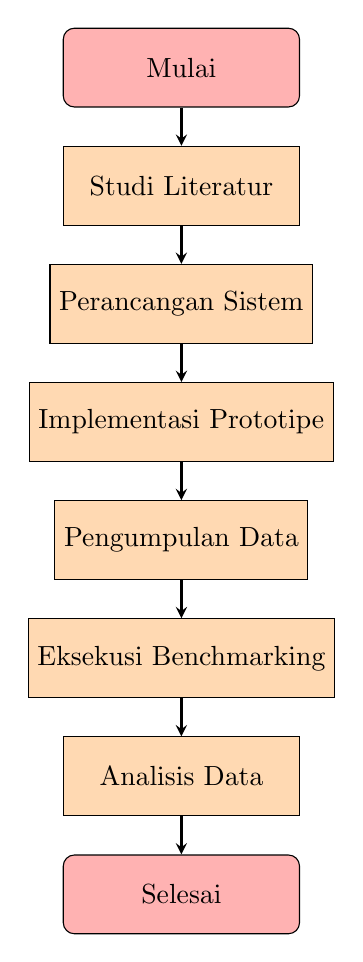
\begin{tikzpicture}[node distance=1.5cm, auto]
        % Define styles
        \tikzstyle{startstop} = [rectangle, rounded corners, minimum width=3cm, minimum height=1cm,text centered, draw=black, fill=red!30]
        \tikzstyle{process} = [rectangle, minimum width=3cm, minimum height=1cm, text centered, draw=black, fill=orange!30]
        \tikzstyle{decision} = [diamond, minimum width=3cm, minimum height=1cm, text centered, draw=black, fill=green!30]
        \tikzstyle{arrow} = [thick,->,>=stealth]

        % Nodes
        \node (start) [startstop] {Mulai};
        \node (lit) [process, below of=start] {Studi Literatur};
        \node (design) [process, below of=lit] {Perancangan Sistem};
        \node (impl) [process, below of=design] {Implementasi Prototipe};
        \node (data) [process, below of=impl] {Pengumpulan Data};
        \node (bench) [process, below of=data] {Eksekusi Benchmarking};
        \node (anal) [process, below of=bench] {Analisis Data};
        \node (end) [startstop, below of=anal] {Selesai};

        % Arrows
        \draw [arrow] (start) -- (lit);
        \draw [arrow] (lit) -- (design);
        \draw [arrow] (design) -- (impl);
        \draw [arrow] (impl) -- (data);
        \draw [arrow] (data) -- (bench);
        \draw [arrow] (bench) -- (anal);
        \draw [arrow] (anal) -- (end);
    \end{tikzpicture}
    }
    \caption{Alur Penelitian (\textit{Flowchart})}
\end{figure}

Berikut adalah penjabaran rinci dari setiap tahapan penelitian:
\begin{enumerate}
    \item \textbf{Studi Literatur:} Melakukan peninjauan mendalam terhadap dokumentasi model \foreign{Whisper}, arsitektur sistem terdistribusi berbasis antrean (\foreign{queue-based}), dan metrik evaluasi ASR. Tahap ini juga mencakup eksplorasi teori \textit{human-computer interaction} untuk mendukung perancangan antarmuka koreksi yang ergonomis. Peneliti mengumpulkan berbagai referensi ilmiah untuk memastikan landasan teori yang digunakan telah sesuai dengan standar akademik terkini.
    \item \textbf{Perancangan Sistem:} Merancang skema interaksi antara \foreign{Next.js} sebagai orkestrator tugas dan \foreign{Python Worker} sebagai unit eksekusi GPU. Perancangan meliputi skema Redis \foreign{Pub/Sub} untuk pelaporan status transkripsi secara \foreign{real-time} serta struktur data laporan hasil benchmarking. Peneliti juga merancang diagram basis data untuk menyimpan informasi pengguna, berkas audio, dan segmen transkripsi.
    \item \textbf{Implementasi Prototipe:} Membangun sistem transkripsi fungsional yang mengintegrasikan seluruh komponen perangkat lunak yang telah direncanakan. \foreign{Worker} dikonfigurasi menggunakan \foreign{Faster-Whisper} untuk memaksimalkan penggunaan VRAM pada RTX A4000 melalui teknik kuantisasi yang tepat. Implementasi ini mencakup pembuatan antarmuka web interaktif yang memungkinkan pengguna untuk mengunggah audio dan memantau progres secara langsung.
    \item \textbf{Pengumpulan Data:} Menyiapkan 11.540 segmen audio dari korpus \foreign{Mozilla Common Voice} beserta berkas \foreign{source-of-truth} transkrip dalam format \foreign{TSV}. Data divalidasi kesesuaiannya antara durasi audio dan teks transkrip manual untuk menghindari bias saat proses evaluasi. Peneliti memastikan keragaman audio dalam hal kebisingan dan kecepatan bicara untuk menguji ketahanan model secara objektif.
    \item \textbf{Eksekusi Benchmarking:} Menjalankan uji coba transkripsi secara berulang untuk varian model \foreign{tiny, base, small, medium, large-v3,} dan \foreign{large-v3-turbo}. Data yang dicatat meliputi waktu inferensi (\textit{Real Time Factor}), penggunaan memori maksimal, dan hasil teks transkripsi mentah. Setiap pengujian dilakukan dalam lingkungan yang terkontrol untuk meminimalisir pengaruh variabel eksternal terhadap hasil pengukuran.
    \item \textbf{Analisis Data \& Dashboard:} Menghitung nilai WER dan CER menggunakan algoritma \foreign{Levenshtein distance} yang diterapkan secara programatik. Hasil analisis divisualisasikan melalui \foreign{dashboard Streamlit} yang menyajikan grafik perbandingan performa antar model secara interaktif. Tahap ini diakhiri dengan penarikan kesimpulan mengenai varian model yang paling optimal untuk diimplementasikan dalam skenario dunia nyata.
\end{enumerate}

\section{Arsitektur Sistem (Skriptor)}
Sistem Skriptor dibangun menggunakan pendekatan arsitektur terdistribusi untuk memisahkan beban kerja antarmuka dari beban kerja inferensi AI yang berat. Desain ini memungkinkan aplikasi tetap responsif meskipun sedang memproses ribuan segmen audio secara simultan di latar belakang.

\subsection{Aplikasi Utama (Next.js Orchestrator)}
Aplikasi utama dikembangkan menggunakan \foreign{Next.js} 16 yang berfungsi sebagai pusat kendali dan antarmuka bagi pengguna akhir. Pemanfaatan \foreign{Partial Prerendering} (PPR) dan \foreign{Server Components} memungkinkan penyajian konten statis secara instan sambil memuat data dinamis secara asinkron di latar belakang. Backend aplikasi menangani manajemen sesi pengguna melalui \foreign{Better Auth} dan interaksi basis data menggunakan \foreign{Drizzle ORM} yang menjamin keamanan tipe data. Aplikasi ini bertanggung jawab untuk menerima unggahan berkas audio, menyimpannya ke penyimpanan \foreign{S3}, dan memasukkan pekerjaan baru ke dalam antrean tugas \foreign{BullMQ}.

\subsection{Worker Transkripsi (Python AI Engine)}
Unit pemrosesan AI diimplementasikan menggunakan bahasa pemrograman Python untuk memanfaatkan ekosistem \textit{deep learning} yang matang dan berperforma tinggi. \textit{Worker} ini berjalan sebagai layanan independen yang terus memantau antrean tugas pada Redis untuk mengeksekusi pekerjaan transkripsi yang masuk. Pustaka \foreign{WhisperX} digunakan untuk proses transkripsi karena dukungannya terhadap penyelarasan tingkat kata (\textit{word-level alignment}) dan diarization pembicara yang akurat. Hasil transkripsi kemudian dikirim kembali ke aplikasi utama melalui \textit{signed callback} berbasis HMAC untuk menjamin integritas data dan keamanan komunikasi antar layanan.

\subsection{Mekanisme Komunikasi asinkron (Redis \& BullMQ)}
Komunikasi antara aplikasi \textit{web} dan \textit{worker} AI dikelola oleh \foreign{Redis} sebagai perantara pesan (\foreign{message broker}) dengan protokol \foreign{BullMQ}. Saat pengguna mengunggah audio, aplikasi utama menciptakan entitas pekerjaan (\foreign{job}) yang berisi metadata audio dan parameter model yang diinginkan. \foreign{BullMQ} mengelola siklus hidup pekerjaan tersebut, termasuk penanganan percobaan ulang (\foreign{retry logic}) jika terjadi kegagalan sistem dan pelaporan progres secara \textit{real-time}. Progres transkripsi dikirimkan kembali ke pengguna melalui \foreign{Server-Sent Events} (SSE), yang memungkinkan pembaruan persentase progres di layar pengguna tanpa perlu melakukan pemuatan ulang halaman secara manual.

\subsection{Antarmuka Koreksi Manual (Human-in-the-Loop UI)}
Antarmuka koreksi manual pada sistem Skriptor dirancang untuk memfasilitasi alur kerja \textit{human-in-the-loop} yang efisien dan presisi. Komponen utama antarmuka ini adalah visualisasi bentuk gelombang audio interaktif menggunakan pustaka \textit{wavesurfer.js} yang tersinkronisasi secara langsung dengan editor teks berbasis komponen. Pengguna dapat menavigasi audio dengan cara mengeklik segmen teks tertentu, sehingga mempermudah proses verifikasi pendengaran terhadap kata-kata yang diragukan akurasinya oleh AI. Editor teks tersebut mendukung fitur pelacakan waktu (\textit{timestamping}) otomatis untuk setiap segmen, yang menjamin konsistensi antara data audio dan teks hasil perbaikan manual. Dengan adanya fitur ini, sistem tidak hanya berfungsi sebagai alat transkripsi otomatis, tetapi juga sebagai platform produktivitas yang menjamin kualitas akhir transkrip mencapai standar profesional.

\section{Teknik Analisis Data}
Data yang terkumpul dianalisis secara kuantitatif untuk menjawab rumusan masalah.

\subsection{Perhitungan Akurasi (WER dan CER)}
Akurasi model diukur menggunakan dua metrik utama berbasis \foreign{Levenshtein Distance}, yaitu \foreign{Word Error Rate} (WER) dan \foreign{Character Error Rate} (CER).

\begin{enumerate}
    \item \textbf{Word Error Rate (WER):} Mengukur kesalahan pada tingkat kata. Rumus WER dinyatakan pada Persamaan (3.1):
    \begin{equation}
        WER = \frac{S + D + I}{N} = \frac{S + D + I}{S + D + C}
    \end{equation}
    Dimana:
    \begin{itemize}
        \item $S$ = \foreign{Substitutions} (kata yang salah diganti).
        \item $D$ = \foreign{Deletions} (kata yang hilang).
        \item $I$ = \foreign{Insertions} (kata tambahan yang tidak ada di referensi).
        \item $C$ = \foreign{Correct words} (kata yang benar).
        \item $N$ = Jumlah total kata pada transkrip referensi.
    \end{itemize}

    \item \textbf{Character Error Rate (CER):} Mengukur kesalahan pada tingkat karakter. Rumusnya identik dengan WER namun diterapkan pada setiap unit karakter. CER sangat penting untuk bahasa dengan variasi morfologi yang kompleks atau untuk melihat ketelitian penulisan ejaan.
\end{enumerate}

\subsection{Analisis Performa Komputasi}
Performa sistem diukur melalui:
\begin{enumerate}
    \item \textbf{Real Time Factor (RTF):} Rasio waktu pemrosesan terhadap durasi audio asli. RTF < 1 menunjukkan kecepatan transkripsi lebih cepat dari durasi audio.
    \item \textbf{VRAM Utilization:} Konsumsi memori kartu grafis maksimal selama proses inferensi untuk menentukan kelayakan model pada perangkat keras tertentu.
\end{enumerate}

\subsection{Sistem Pelaporan dan Visualisasi}
Hasil akhir penelitian disajikan dalam tiga format utama untuk memastikan transparansi dan kemudahan akses data:
\begin{enumerate}
    \item \textbf{Streamlit Dashboard:} Aplikasi interaktif untuk memvisualisasikan grafik perbandingan WER/CER antar model, distribusi penggunaan VRAM, dan korelasi antara panjang audio dengan waktu transkripsi.
    \item \textbf{Laporan Terstruktur (Markdown):} Dokumen penjelasan hasil analisis untuk setiap varian model yang berisi kesimpulan kualitatif dari data kuantitatif.
    \item \textbf{Raw Data (Excel/XLSX):} Kumpulan data mentah hasil benchmarking untuk setiap segmen audio guna memungkinkan verifikasi ulang oleh pihak lain.
\end{enumerate}
